354. \begin{figure}[ht!]
\center{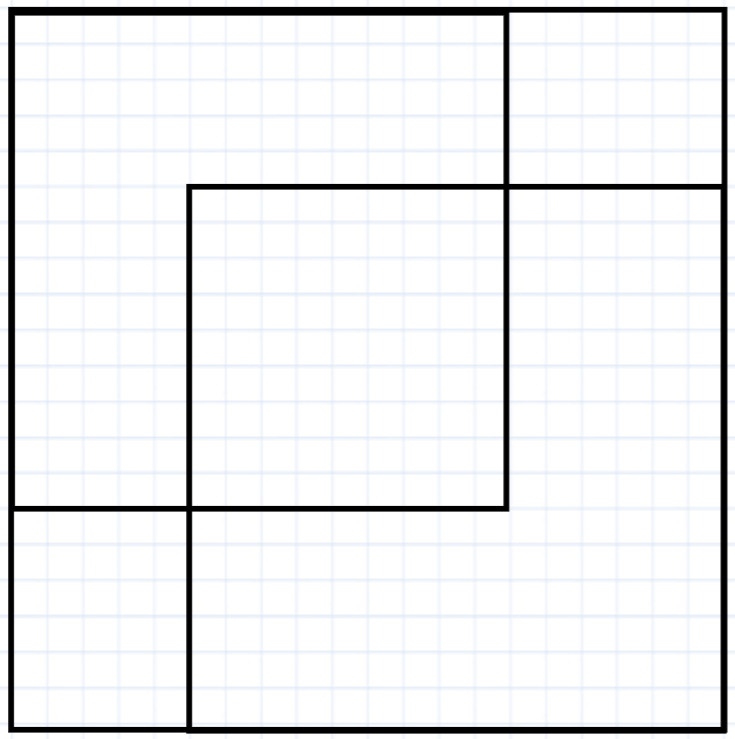
\includegraphics[scale=0.35]{kovr1.png}}
\end{figure}\\
Наименьшая площадь будет покрыта сразу двумя коврами в том случае, когда они лежат в противоположных углах комнаты. В этом случае они вместе покрывают квадрат размером $10\times10$ метров, его площадь равна $10\cdot10=100\text{ м}^2.$\\
